\newcommand{\paneltitlefont}{\fontsize{6.75}{7}\selectfont}
\newcommand{\paneltextfont}{\fontsize{5}{4}\selectfont}
\newcommand{\panelcaptionfont}{\fontsize{5.5}{7}\selectfont}

\fontfamily{LinuxLibertineT-LF}\selectfont
\color{black!95}

\vspace{2mm}

{\paneltitlefont C. Replicates diverge\par}

\vspace{0.2em}

\noindent\makebox[\linewidth][c]{%
    \begin{minipage}{0.82\linewidth}
        \centering
        \paneltextfont
        Distribution of allele frequencies\\
        across replicate populations
    \end{minipage}%
}
\par

\vspace{0.1em}

\noindent\makebox[\linewidth][c]{%
    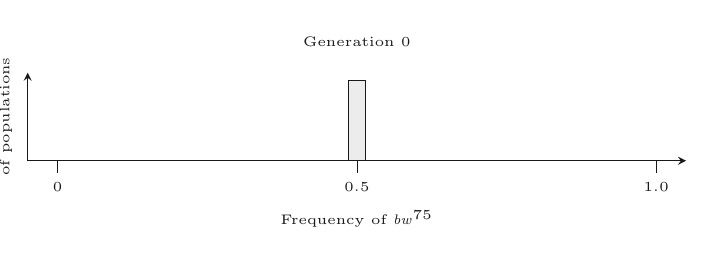
\begin{tikzpicture}[trim axis left,trim axis right]
    \begin{axis}[
        width=0.82\linewidth,
        height=2.7cm,
        title={Generation 0},
        title style={
            font=\paneltextfont,
            text=black!90
        },
        xmin=-0.05,
        xmax=1.05,
        ymin=0,
        ymax=1.1,
        xtick={0,0.5,1},
        xticklabels={$0$,$0.5$,$1.0$},
        ytick=\empty,
        xlabel={Frequency of \textit{bw}\textsuperscript{75}},
        ylabel={Relative number\\of populations},
        ylabel style={
            align=center,
            font=\paneltextfont,
            text=black!90
        },
        xlabel style={
            font=\paneltextfont,
            text=black!90
        },
        tick label style={
            font=\paneltextfont,
            text=black!90
        },
        axis lines=left,
        axis line style={
            draw=black!90,
            line width=0.3pt
        },
        tick style={
            draw=black!90,
            line width=0.25pt
        },
        font=\paneltextfont,
        ybar,
        bar width=6pt,
        enlarge x limits=false
    ]
        \addplot[
            fill=gray!15,
            draw=black!90,
            line width=0.3pt
        ]
        coordinates {
            (0.5,1)
        };
    \end{axis}
\end{tikzpicture}
}
\par

% \vspace{-1.1em}

\noindent\makebox[\linewidth][c]{%
    {\fontsize{7}{7}\selectfont\color{black!80}$\downarrow$}%
}
\par

% \vspace{-0.8em}

\noindent\makebox[\linewidth][c]{%
    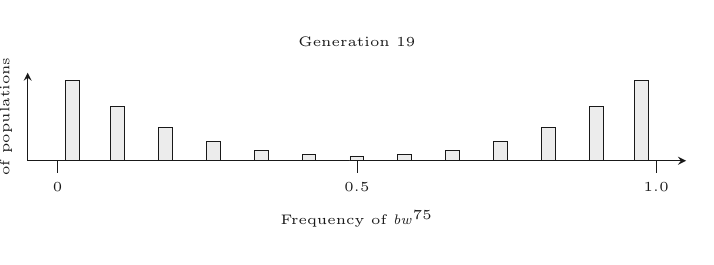
\begin{tikzpicture}[trim axis left,trim axis right]
    \begin{axis}[
        width=0.82\linewidth,
        height=2.7cm,
        title={Generation 19},
        title style={
            font=\paneltextfont,
            text=black!90
        },
        xmin=-0.05,
        xmax=1.05,
        ymin=0,
        ymax=1.1,
        xtick={0,0.5,1},
        xticklabels={$0$,$0.5$,$1.0$},
        ytick=\empty,
        xlabel={Frequency of \textit{bw}\textsuperscript{75}},
        ylabel={Relative number\\of populations},
        ylabel style={
            align=center,
            font=\paneltextfont,
            text=black!90
        },
        xlabel style={
            font=\paneltextfont,
            text=black!90
        },
        tick label style={
            font=\paneltextfont,
            text=black!90
        },
        axis lines=left,
        axis line style={
            draw=black!90,
            line width=0.3pt
        },
        tick style={
            draw=black!90,
            line width=0.25pt
        },
        font=\paneltextfont,
        ybar,
        bar width=5pt,
        enlarge x limits=false
    ]
        \addplot[
            fill=gray!15,
            draw=black!90,
            line width=0.3pt
        ]
        coordinates {
            (0.025,1.00)
            (0.10,0.68)
            (0.18,0.42)
            (0.26,0.24)
            (0.34,0.13)
            (0.42,0.08)
            (0.50,0.06)
            (0.58,0.08)
            (0.66,0.13)
            (0.74,0.24)
            (0.82,0.42)
            (0.90,0.68)
            (0.975,1.00)
        };
    \end{axis}
\end{tikzpicture}
}
\par

\vspace{0.6em}

\noindent\makebox[\linewidth][c]{%
    \begin{minipage}{0.82\linewidth}
        \centering
        \panelcaptionfont
        Genetic drift causes replicate populations to follow different paths even without selection.
    \end{minipage}
}
\par